% Task-family x agent PASS rate (%), visualized as a green heatmap.
% Values derived from reports/eval_scores_v2_long.csv, majority-of-4 voting.
\begin{figure}[t]
\centering
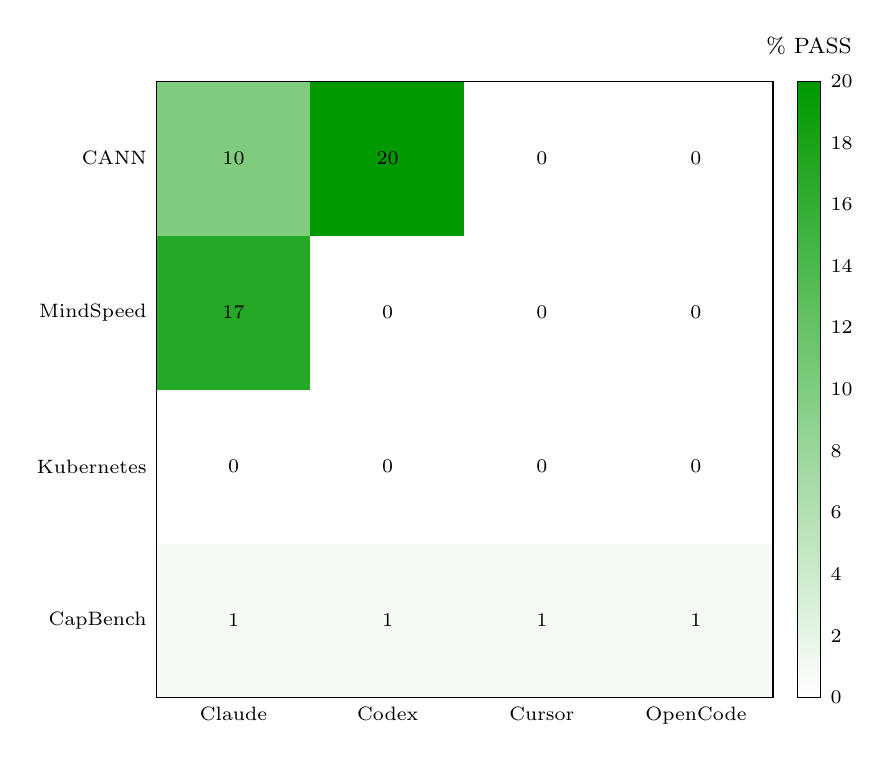
\begin{tikzpicture}
\begin{axis}[
    colormap={gr}{color=(white) color=(green!60!black)},
    colorbar,
    colorbar style={
      width=3mm,
      title={\footnotesize \% PASS},
      yticklabel style={font=\scriptsize},
    },
    point meta min=0, point meta max=20,
    xtick={0,1,2,3},
    xticklabels={Claude, Codex, Cursor, OpenCode},
    ytick={0,1,2,3},
    yticklabels={CapBench, Kubernetes, MindSpeed, CANN},
    tick style={draw=none},
    axis on top,
    enlargelimits=false,
    axis equal image,
    width=0.9\linewidth,
    xticklabel style={font=\scriptsize},
    yticklabel style={font=\scriptsize},
    nodes near coords,
    nodes near coords style={font=\scriptsize},
    nodes near coords align=center,
    point meta=explicit symbolic,
    every node near coord/.append style={yshift=0mm}
  ]
    \addplot[
      matrix plot*,
      mesh/cols=4,
      point meta=explicit,
      shader=flat corner,
    ] table[meta=v] {
      x y v
      0 0 1
      1 0 1
      2 0 1
      3 0 1
      0 1 0
      1 1 0
      2 1 0
      3 1 0
      0 2 17
      1 2 0
      2 2 0
      3 2 0
      0 3 10
      1 3 20
      2 3 0
      3 3 0
    };
  \end{axis}
  \end{tikzpicture}
  \caption{Pass rate (\%) by agent and task family under the majority-of-4 verdict. Rows top-to-bottom: \emph{CANN}, \emph{MindSpeed}, \emph{Kubernetes}, \emph{CapBench}. Kubernetes (K1--K4) is a \emph{uniform zero-pass} cliff across all agents.}
\label{fig:pass-heatmap}
\end{figure}
